\documentclass[11pt]{article}
\usepackage[utf8]{inputenc}	% Para caracteres en español
\usepackage{amsmath,amsthm,amsfonts,amssymb,amscd}
\usepackage{multirow,booktabs}
\usepackage[table]{xcolor}
\usepackage{fullpage}
\usepackage{lastpage}
\usepackage{enumitem}
\usepackage{fancyhdr}
\usepackage{mathrsfs}
\usepackage{wrapfig}
\usepackage{setspace}
\usepackage{hyperref}
\usepackage{calc}
\usepackage{multicol}
\usepackage{cancel}
\usepackage[retainorgcmds]{IEEEtrantools}
\usepackage[margin=3cm]{geometry}
\usepackage{amsmath}
\newlength{\tabcont}
\setlength{\parindent}{0.0in}
\setlength{\parskip}{0.05in}
\usepackage{empheq}
\usepackage{framed}
\usepackage[most]{tcolorbox}
\usepackage{xcolor}
\colorlet{shadecolor}{orange!15}
\parindent 0in
\parskip 12pt
\geometry{margin=1in, headsep=0.25in}
\theoremstyle{definition}
\usepackage{pdfpages}
\newtheorem{defn}{Definition}
\newtheorem{reg}{Rule}
\newtheorem{exer}{Exercise}
\newtheorem{note}{Note}
\usepackage{fancyhdr}\usepackage{xcolor}\usepackage{amsmath}\usepackage{amssymb}\pagestyle{fancy}\rhead{}
\newtheorem{theorem}{Theorem}[subsection]
\theoremstyle{definition}
\newtheorem{definition}[theorem]{Definiton}
\newtheorem{example}[theorem]{Example}
\newtheorem{corollary}[theorem]{Corollary}
\newtheorem{lemma}[theorem]{Lemma}
\title{Chapter 9 Review Notes}
\begin{document}
\thispagestyle{empty}
{\LARGE \bf ESC 195 Lecture Notes}\\
{\large Hei Shing Cheung}\\
Caculus II, Winter 2024 \hfill ESC 195\\
\section{More on Integrals}
\subsection{Riemann Sum - Non-Uniform Petition}
\begin{example}
    Given the following definite integral:
    $$\int^2_0 \sqrt{x} dx$$, we cannot evaluate its Riemann sum with uniforms partition, since the series of root cannot be easily evaluated. 
\end{example}

The definite integral of $\sqrt{x}$ from $0$ to $2$ using a Riemann sum with a non-uniform partition is given by:

$$
\int_{0}^{2} \sqrt{x} \, dx = \lim_{n \to \infty} \sum_{i=1}^n \sqrt{x_i} \Delta x_i
$$

where:
\begin{itemize}
    \item $x_0 = 0, \, x_n = 2$,
    \item $x_i = i^2 \cdot \frac{2}{n^2}$ for $i = 0, 1, 2, \dots, n$,
    \item $\Delta x_i = x_i - x_{i-1} = \frac{2}{n^2} \cdot (2i - 1)$.
\end{itemize}

The Riemann sum becomes:
$$
S_n = \sum_{i=1}^n \sqrt{i^2 \cdot \frac{2}{n^2}} \cdot \frac{2}{n^2} \cdot (2i - 1).
$$

Simplifying further:
$$
S_n = \sum_{i=1}^n \sqrt{\frac{2i^2}{n^2}} \cdot \frac{2}{n^2} \cdot (2i - 1).
$$

Taking the limit as $n \to \infty$, the sum converges to the exact value of the integral using the series of squares. 
$$
\int_{0}^{2} \sqrt{x} \, dx = \frac{4\sqrt{2}}{3}.
$$
\paragraph{Condition} $n \to \infty$ Ensures $\Delta x_i \to 0$
\paragraph{} As $n \to \infty$, the partition points $x_i$ become increasingly dense. This ensures that the partition becomes infinitely fine.

\subsection{Integration By Parts}
Using the product rule:
$$
\frac{d}{dx} \big[ u(x) v(x) \big] = u'(x)v(x) + u(x)v'(x),
$$
integrating both sides with respect to $x$ gives:
$$
u(x)v(x) = \int u'(x) v(x) \, dx + \int u(x) v'(x) \, dx.
$$
Rearranging this:
$$
\int u'(x) v(x) \, dx = u(x)v(x) - \int u(x) v'(x) \, dx.
$$

\paragraph{Integration by parts formula}
\begin{equation}
\int u \, dv = uv - \int v \, du.
\end{equation}
\begin{example}
We want to solve the integral $$ \int x e^{2x} \, dx $$ using integration by parts.

Let:
$$ u = x, \quad dv = e^{2x} \, dx. $$

Then, we compute the derivatives and integrals:
$$ du = dx, \quad v = \frac{e^{2x}}{2}. $$

Now, apply the integration by parts formula:
$$ \int u \, dv = uv - \int v \, du. $$

Substituting in the values:
$$ \int x e^{2x} \, dx = x \cdot \frac{e^{2x}}{2} - \int \frac{e^{2x}}{2} \, dx. $$

Next, compute the remaining integral:
$$ \int \frac{e^{2x}}{2} \, dx = \frac{e^{2x}}{4}. $$

Thus, the result is:
$$ \int x e^{2x} \, dx = \frac{x e^{2x}}{2} - \frac{e^{2x}}{4} + C. $$

\end{example}

\begin{example}
We want to solve $$ \int x^2 \sin(2x) \, dx $$ using double integration by parts.

First, let:
$$ u = x^2, \quad dv = \sin(2x) \, dx. $$

Then:
$$ du = 2x \, dx, \quad v = -\frac{1}{2} \cos(2x). $$

Using the IBP formula:
$$ \int u \, dv = uv - \int v \, du, $$

we get:
$$ \int x^2 \sin(2x) \, dx = -\frac{x^2}{2} \cos(2x) + \int x \cos(2x) \, dx. $$

Now, apply IBP again to \( \int x \cos(2x) \, dx \), let:
$$ u = x, \quad dv = \cos(2x) \, dx. $$

Then:
$$ du = dx, \quad v = \frac{1}{2} \sin(2x). $$

Using the IBP formula again:
$$ \int x \cos(2x) \, dx = \frac{x}{2} \sin(2x) - \int \frac{1}{2} \sin(2x) \, dx, $$

and solving the remaining integral:
$$ \int \frac{1}{2} \sin(2x) \, dx = -\frac{1}{4} \cos(2x). $$

Thus, the final result is:
$$ \int x^2 \sin(2x) \, dx = -\frac{x^2}{2} \cos(2x) + \frac{x}{2} \sin(2x) + \frac{1}{4} \cos(2x) + C. $$

\end{example}
\subsection{Trigonometric Integrals}
\paragraph{Case I} This is the case I trigonometric integrals, the strategy is using the pythagorean identity.
\paragraph{} We want to solve the class of integrals:
\begin{equation}
 \int \sin^n(x) \cos^m(x) \, dx
\end{equation}
, where $m$ or $n$ is odd.
\begin{example}
We want to solve the integral:
$$ I = \int \sin^3(x) \cos^2(x) dx $$
We use the identity: $ \sin^2(x) = 1 - \cos^2(x)$. Thus, the integral becomes:
\begin{align*}
    I &= \int \sin(x)(1 - \cos^2(x)) \cos^2(x) \, dx \\
    &= \int (\cos^2(x) \sin(x) - \cos^4(x) \sin(x)) \, dx
\end{align*} 
which is now easily solvable with substution $u=\cos(x)$.
\end{example}
\paragraph{Case II} The follwoing is generally solvable via case I and case III below. In general, we solve the integral by reducing the power of the trigonometric functions to arrive at a solvable integral Case I or III.
\paragraph{} We want to solve the class of integrals:
\begin{equation} \int \sin^n(x) \cos^m(x) \, dx \end{equation}
, where $m$ and $n$ is even.
\begin{example}
We want to solve the integral:
$$ I = \int \sin^2(x) \cos^4(x) \, dx $$
We can apply the double angle formulas:
\begin{align}
    \sin(x)\cos(x) &= \frac{1}{2} \sin(2x) \\
    \sin^2(x) &= \frac{1 - \cos(2x)}{2} \\
    \cos^2(x) &= \frac{1 + \cos(2x)}{2}
\end{align}
Thus, the integral becomes:
$$ I = \frac{1}{8} \int \sin^2(2x) \, dx + \frac{1}{8} \int \cos(2x)\sin^2(2x) \, dx $$
\end{example}
\paragraph{Case III} This is the case III trigonometric integrals, the strategy is using the reduction formula via IBP.
\paragraph{Reduction Formula} We can solve integrals by reducing the power of the trigonometric functions. These are done using IBP and trigonometric identities.
\paragraph{} We want to solve the classes of integrals:
\begin{equation} 
    \int \sin^n(x) \, dx, \quad \int \cos^n(x) \, dx 
\end{equation}
, where $n$ is a positive integer. For demonstartion, We can obtain the reduction formula of $\sin^n(x)$ via IBP.
\begin{align*}
    I_n &= \int \sin^n(x) \, dx \\
    &= \int \sin^{n-1}(x) \sin(x) \, dx \\
    &= \frac{-\cos(x) \sin^{n-1}(x)}{n} + \frac{(n-1)}{n} \int \cos^2(x) \sin^{n-2}(x) \, dx \\
    &= \frac{-\cos(x) \sin^{n-1}(x)}{n} + \frac{(n-1)}{n} I_{n-2}
\end{align*}
\paragraph{Case IV} The following is generally solvable via simple trigonometric integrals. In general, we solve the integral by applying the angle sum formulas.
\paragraph{} We want to solve the classes of integrals:
\begin{equation}
    \int \sin(mx) \cos(nx) \, dx, \quad \int \sin(mx) \sin(nx) \, dx, \quad \int \cos(mx) \cos(nx) \, dx 
\end{equation}
We could apply the angle sum formulas:
\begin{align}
    \sin(mx)\cos(nx) &= \frac{1}{2} \left[ \sin((m+n)x) + \sin((m-n)x) \right] \\
    \sin(mx)\sin(nx) &= \frac{1}{2} \left[ \cos((m-n)x) - \cos((m+n)x) \right] \\
    \cos(mx)\cos(nx) &= \frac{1}{2} \left[ \cos((m-n)x) + \cos((m+n)x) \right]
\end{align}
\paragraph{Case V} The following is generally solvable via the following trigonometric identities listed below, which convert it into a reduction formula.
\begin{align}
    \tan^2(x) &= \sec^2(x) - 1 \label{eq:tan2} \\
    \cot^2(x) &= \csc^2(x) - 1 \label{eq:cot2}  \\
    \frac{d}{dx} \tan(x) &= \sec^2(x)
\end{align}
\paragraph{} We want to solve the classes of integral:
\begin{equation}
    \int \tan^n(x) \, dx, \quad \int \cot^n(x) \, dx 
\end{equation}
We know that $tan^2(x) = \sec^2(x) - 1$. Thus, we can solve the integral by reducing the power of the tangent function.
\paragraph{Case VI} The following is generally solvable via the trigonometric identities (\ref{eq:tan2}) and (\ref{eq:cot2}).
\paragraph{} We want to solve the classes of integral:
\begin{equation} 
    \int \tan^m(x) \sec^n(x) \, dx, \quad \int \cot^m(x) \csc^n(x) \, dx 
\end{equation}
We can solve the integral by reducing the power of the converted trigonometric functions using (\ref{eq:tan2}) and (\ref{eq:cot2}).
\paragraph{Case VII} The following is generally solvable via the trigonometric identities (\ref{eq:tan2}) and (\ref{eq:cot2}).
\paragraph{} We want to solve the classes of integral:
\begin{equation} \int \tan^m(x) \sec^n(x) \, dx, \quad \int \cot^m(x) \csc^n(x) \, dx \end{equation}
We can solve the integral by converting between the tangent and secant functions using the trigonometric identities.
\paragraph{Case VIII} This is the case VIII integrals, the strategy is using the trigonometric substitution.
\paragraph{Trigonometric Substitution} We can solve integrals by substituting the trigonometric functions with other trigonometric functions.
\begin{example}
We want to solve the integral:
$$ \int \frac{dx}{\sqrt{1 - x^2}} $$
\end{example}
We can substitute $x = \sin(\theta)$, then $dx = \cos(\theta) \, d\theta$. The integral becomes:
$$ \int \frac{\cos(\theta) \, d\theta}{\sqrt{1 - \sin^2(\theta)}} = \int \frac{\cos(\theta) \, d\theta}{\cos(\theta)} = \int d\theta = \theta + C. $$
\paragraph{} In general, we can use the following substitutions:
\begin{itemize}
    \item $x = a\sin(\theta)$ for $\sqrt{a^2 - x^2}$,
    \item $x = a\tan(\theta)$ for $\sqrt{a^2 + x^2}$,
    \item $x = a\sec(\theta)$ for $\sqrt{x^2 - a^2}$.
\end{itemize}
\paragraph{Summary} We can solve trigonometric integrals by using the following strategies:
\begin{table}[h!]
    \centering
    \begin{tabular}{|c|l|}
    \hline
    \textbf{Case} & \textbf{Strategy and General Form} \\ \hline
    I   & Use \(\sin^2(x) + \cos^2(x) = 1\); simplify using substitution. \\
        & General Form: \(\int \sin^n(x) \cos^m(x) dx\), where \(m\) or \(n\) is odd. \\ \hline
    II  & Convert to Case I and Case III using double angle formulas. \\
        & General Form: \(\int \sin^n(x) \cos^m(x) dx\), where both \(m\) and \(n\) are even. \\ \hline
    III & Apply reduction formulas derived via integration by parts. \\
        & General Form: \(\int \sin^n(x) dx\) or \(\int \cos^n(x) dx\). \\ \hline
    IV  & Use angle sum formulas to simplify. \\
        & General Form: \(\int \sin(mx) \cos(nx) dx\). \\ \hline
    V   & Reduce tangent/cotangent powers using \(\tan^2(x) = \sec^2(x) - 1\) and substitution. \\
        & General Form: \(\int \tan^n(x) dx\) or \(\int \cot^n(x) dx\). \\ \hline
    VI  & Convert to Case V via Pythagorean identities. \\
        & General Form: \(\int \tan^m(x) \sec^n(x) dx\) or \(\int \cot^m(x) \csc^n(x) dx\). \\ \hline
    VII & Convert between tangent and secant functions for simplification. \\
        & General Form: \(\int \tan^m(x) \sec^n(x) dx\). \\ \hline
    VIII & Use trigonometric substitution: \(x = a \sin(\theta), a \tan(\theta), a \sec(\theta)\). \\
         & General Form: \(\int \frac{dx}{\sqrt{a^2 - x^2}}, \int \frac{dx}{\sqrt{a^2 + x^2}}, \int \frac{dx}{\sqrt{x^2 - a^2}}\). \\ \hline
    \end{tabular}
    \caption{Strategies and General Forms for Case I-VIII Integrals}
\end{table}

\section{Hyperbolic Trigonometric Functions}
\begin{definition}[Hyperbolic Sine]
    The hyperbolic sine function is defined as:
    \begin{equation} \sinh(x) = \frac{e^x - e^{-x}}{2}. \end{equation}
\end{definition}
\begin{definition}[Hyperbolic Cosine]
    The hyperbolic cosine function is defined as:
    \begin{equation}  \cosh(x) = \frac{e^x + e^{-x}}{2}. \end{equation}
\end{definition}
\paragraph{Properties} These combinations of exponential functions have properties similar to the trigonometric functions.
\paragraph{Derivatives} The derivatives of the hyperbolic functions are:
\begin{align}
    \frac{d}{dx} \sinh(x) &= \cosh(x), \\
    \frac{d}{dx} \cosh(x) &= \sinh(x).
\end{align}
\paragraph{Identities} The hyperbolic functions satisfy the following identities:
\begin{align}
    \cosh^2(x) - \sinh^2(x) &= 1, \\
    \cosh(2x) &= \cosh^2(x) + \sinh^2(x), \\
    \sinh(2x) &= 2\sinh(x)\cosh(x).
\end{align}
\paragraph{Hyperbola} The hyperbolic functions are related to the hyperbola $x^2 - y^2 = 1$. Simiar to the circle, the hyperbola can be parametrized by the hyperbolic functions (e.g. $x = \cosh(t)$, $y = \sinh(t)$).
\paragraph{Area} The area of a sector of the hyperbola is given by:
\begin{equation}
    A = t/2,
\end{equation} 
where $t$ is the angle of the sector along the parametrization $\{(x,y)\mid x = \cosh(t), y = \sinh(t)\}$.
\begin{figure}[h!]
    \begin{center}
        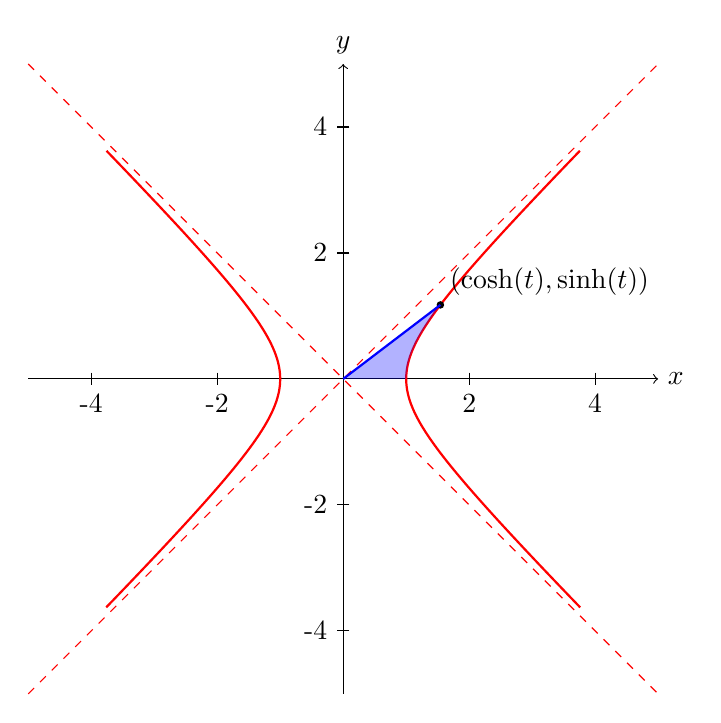
\begin{tikzpicture}[scale=0.8]
            % Draw the axes
            \draw[->] (-5, 0) -- (5, 0) node[right] {$x$};
            \draw[->] (0, -5) -- (0, 5) node[above] {$y$};
        
            % Draw ticks on the axes
            \foreach \x in {-4, -2, 2, 4}
                \draw (\x, 0.1) -- (\x, -0.1) node[below] {\x};
            \foreach \y in {-4, -2, 2, 4}
                \draw (0.1, \y) -- (-0.1, \y) node[left] {\y};
        
            % Draw the hyperbola branches
            \draw[thick, red, domain=-2:2, samples=100] plot ({cosh(\x)}, {sinh(\x)});
            \draw[thick, red, domain=-2:2, samples=100] plot ({-cosh(\x)}, {sinh(\x)});
        
            % Draw the asymptotes
            \draw[red, dashed] (-5, -5) -- (5, 5);
            \draw[red, dashed] (-5, 5) -- (5, -5);
        
            % Add a point on the hyperbola
            \coordinate (P) at ({cosh(1)}, {sinh(1)});
            \draw[fill] (P) circle (0.05) node[above right] {$(\cosh(t), \sinh(t))$};
        
            % Connect the labeled point to the origin
            \draw[thick, blue] (0, 0) -- (P);
        
            % Fill the sector area between hyperbola, line, and x-axis
            \fill[blue, opacity=0.3, domain=0:1, variable=\t]
                (0, 0) -- plot ({cosh(\t)}, {sinh(\t)}) -- cycle;
        \end{tikzpicture}
    \end{center}
    \caption{Sector of the hyperbola}
    \centering
\end{figure}
\paragraph{Catenary} The hyperbolic cosine function describes the shape of a hanging chain or cable. The catenary is the curve formed by a chain hanging from two points. It is given by the equation:
\begin{equation}
    a \cosh\left(\frac{x}{a}\right),
\end{equation}
\begin{definition}[Hyperbolic Tangent]
    The hyperbolic tangent function is defined as:
    \begin{equation}
        \tanh(x) = \frac{\sinh(x)}{\cosh(x)} = \frac{e^x - e^{-x}}{e^x + e^{-x}}. 
    \end{equation}
\end{definition}
\paragraph{Derivative} The derivative of the hyperbolic tangent function resembles the derivative of the regular tangent function:
\begin{equation} \frac{d}{dx} \tanh(x) = \text{sech}^2(x). \end{equation}
\paragraph{Identities} The hyperbolic tangent function satisfies the following identities:
\begin{align}
    \tanh(x) &= \frac{\sinh(x)}{\cosh(x)}, \\
    \text{sech}^2(x) &= 1 - \tanh^2(x).
\end{align}
\paragraph{Secant, Cosecant, Cotangent} The hyperbolic secant, cosecant, and cotangent functions are defined similarly to the regular secant, cosecant, and cotangent functions. They are the \textbf{reciprocal} of the hyperbolic cosine, sine, and tangent functions, respectively.
\paragraph{Inverse Hyperbolic Functions} The inverse hyperbolic functions are defined as the inverse of the hyperbolic functions. They are denoted by $\sinh^{-1}(x)$, $\cosh^{-1}(x)$, $\tanh^{-1}(x)$, etc.
\begin{align}
    \text{arsinh } x &= \ln\left(x + \sqrt{x^2 + 1}\right) \\[10pt]
    \text{arcosh } x &= \ln\left(x + \sqrt{x^2 - 1}\right) \\[10pt]
    \text{artanh } x &= \frac{1}{2} \ln\left(\frac{1 + x}{1 - x}\right) \\[10pt]
    \text{arcsch } x &= \ln\left(\frac{1}{x} + \sqrt{\frac{1}{x^2} + 1}\right) \\[10pt]
    \text{arsech } x &= \ln\left(\frac{1}{x} + \sqrt{\frac{1}{x^2} - 1}\right) \\[10pt]
    \text{arcoth } x &= \frac{1}{2} \ln\left(\frac{x + 1}{x - 1}\right)
\end{align}

\end{document}
